\label{sec:ex}

\section{Introduction}
In this Section, we analyze the behavior
of the grid and  cubature methods on a real landscape.
First, we compare the results calculated with different 
parameterisations 
of each  method; then,
 the two methods are compared.

\subsection{Data}
The data are 66 polygons extracted from
the ORTHO demo, a IGN\footnote{Institut Géographique National:
  \href{http://www.ign.fr/rubrique.asp?rbr\_id=1619}
{http://www.ign.fr/rubrique.asp?rbr\_id=1619}} data base
, see~Fig.~\ref{fig:parcelle}.
\begin{figure}
  \begin{center}
    \includegraphics[angle=-90, width=15cm]{./VignetteDir/graphics/parcelles.ps}
  \end{center}
\caption{Example of 66  polygons extracted from the ORTHO IGN data base. Unit is meter.}\label{fig:parcelle}
\end{figure}
To illustrate  contrasted situations,
five pairs of polygons are treated:
\begin{itemize}
\item
\textbf{(1,1)}: two identical convex polygons,
\item
\textbf{(14,14)}: two identical non-convex polygons,
\item
\textbf{(11,12)}: two convex polygons next to each other,
\item
\textbf{(56,57 )}: two polygons next to each other, one  convex, the
other non-convex,
\item
\textbf{(4,4)}: two identical very irregular polygons.
\end{itemize}
The individual dispersal function is
the oilseed rape pollen dispersal function
defined in~Section~\ref{pollen:funct}.


\section{Influence of the parameterisation in the grid method}


In the grid method, two parameters must be chosen
according to the user's needs:
 the number of
replications and  the grid step.

\subsection{Influence of the number of replications}

To compare the results calculated with different numbers of
replications, 
four values were successively applied:
$r=$ 5, 10, 15, 20. The grid step was constant and equal to 1~m
for both axes.

The results\footnote{Results are dependent on the random numbers generator; so,
actual values may be slightly different.} 
are given in~Table~\ref{array:nr}.
They are:
the evaluated mean flow ($\widehat{\A}$),
the standard deviation ($\widehat\sigma$),
 the coefficient of variation ($\widehat\sigma/\widehat{\A}$)
and the execution time\footnote{
Execution times depend on the material context.
They have been observed here on a Dell Biprocessor, in shared mode
and 3,2GhZ.}.
We can notice that 
the execution times are the
longer as the polygons are the more irregular:
calculation is faster on convex polygons 
(1$\leftrightarrow$1, 11$\leftrightarrow$12) than on non convex ones
(14$\leftrightarrow$14, 56$\leftrightarrow$57)
and very much longer on irregular polygons (4$\leftrightarrow$4).


\begin{table}
\footnotesize
\caption{\label{array:nr} Grid results  with different
  numbers of replications ($r$) and grid step equal to 1~m.}
\begin{center}
\begin{tabular}{|p{1.5cm}|p{1.5cm}|p{1.5cm}|p{1.5cm}|p{1.5cm}|p{1.2cm}|}
\hline
\textbf{Polygons} & 
$r$ & $\widehat{\A}$ &
$\widehat\sigma$ & $\widehat\sigma/\widehat{\A}\times$100  & $Times$
 \\ \hline
1$\leftrightarrow$1 & 5 & 12222.2  & 234.6 & 1.88 & 3.5\\
 & 10   & 12282.5  & 217.7 & 1.77 &  7.0 \\
 & 15 & 12238.8  &  204.1 & 1.66 & 10.5 \\
 & 20 &  12247.7  &  220.9 & 1.80 & 14.1
 \\ \hline
14$\leftrightarrow$14&  5 &  23542.1  & 461.6   & 1.96 & 31.9 \\
 &  10   &  23359.0   & 391.1 & 1.67 & 63.7\\
&  15 & 23411  &  344.4  & 1.47 & 95.3\\
& 20 &  23413.3  & 332.4 & 1.41 & 126.7
 \\ \hline
11$\leftrightarrow$12 &  5 & 164.5  & 2.4 & 1.48 & 7.0 \\
 &  10   & 166.1  & 3.1 & 1.89 & 14.0\\
&  15 & 167.3  & 3.1 & 1.85 & 21.1 \\
& 20 & 167.2  & 3.1 & 1.84 & 27.9
 \\ \hline
56$\leftrightarrow$57 &  5 & 132.5  & 2.0 & 1.51 & 5.9 \\
&  10   & 133.0  & 2.2 & 1.70 & 11.7\\
& 15 &  132.5  & 2.1 & 1.62 &  17.6\\
& 20 & 132.8  & 1.9 & 1.49 & 23.4
 \\ \hline
4$\leftrightarrow$4 &  5 & 14610.1  & 72.3 & 0.5 & 45.7 \\
 & 10   & 14570.9  & 91.5 & 0.62 & 90.7\\
&  15 & 14617.7  & 155.2 & 1.06 & 136.7\\
& 20 &14631.5  & 151.5 & 1.03 & 181.2
 \\ \hline
\end{tabular}
\end{center}
\normalsize
\end{table}



\subsection{Influence of the grid step}


To compare the results calculated with different grid steps, 
four values were tried successively:
$step=$~0.25~m,~0.5~m,~0.75~m~and~1~m.
The number of replications, $r$, is set to 10.

The results are displayed in Table~\ref{array:step}.
As expected, 
the  times  increase
 as the steps become smaller.

\begin{table}
\footnotesize
\caption{\label{array:step} Grid results  with different steps
($r=10$);}
\begin{center}
\begin{tabular}{|p{1.5cm}|p{1.5cm}|p{1.5cm}|p{1.5cm}|p{1cm}|p{1.5cm}|}
\hline
\textbf{Polygons} & $step$ & $\widehat{\A}$ &
$\widehat\sigma$ & $\widehat\sigma/\widehat{\A}\times$100  & $Times$
 \\ \hline
1$\leftrightarrow$1  
 & 1   & 12282.5  & 217.7 & 1.77 &  7.0\\
& 0.75 & 12196.9  & 27.3 & 0.22 & 12.6 \\
& 0.5 & 12277  &  32.8 & 0.26 & 28.5\\
& 0.25 & 12273.8   & 4.08 & 0.03 & 111.5\\
\hline
14$\leftrightarrow$14
 &  1   & 23359.0  & 391.1 & 1.67 & 63.7\\
& 0.75 & 23362.7  &183.2 & 0.78 & 114.5\\
& 0.5 &23376.7  & 63.4 & 0.27 & 258.5\\
 & 0.25 & 23380.6   & 7.7 & 0.03 & 1016.6\\
 \hline
11$\leftrightarrow$12
 &  1   & 166.1  & 3.1 & 1.89 & 14.0\\
& 0.75 & 167.2   & 1.4 & 0.85 & 25.3\\
& 0.5 & 167.1  & 0.5 & 0.34 & 57.1\\
 & 0.25 & 167.2 & 0.1 & 0.05 & 223.9 \\
 \hline
56$\leftrightarrow$57
&  1   & 133.0  & 2.26 & 1.70 & 11.7\\
& 0.75 & 132.5  & 0.87 & 0.66 & 21.1\\
& 0.5 & 132.5  & 0.32 & 0.24 & 47.8\\
 &0.25 &  132.5  & 0.02 & 0.02 & 187.5\\
 \hline
4$\leftrightarrow$4
 & 1   & 14570.9 & 91.5 & 0.62 & 90.7\\
& 0.75 & 14585.4  & 46.9 & 0.32 &  164.5\\
& 0.5 & 14607.7   & 14.8 & 0.10 & 370.9\\
 & 0.25 & 14612.8  & 1.85 & 0.01 & 1452.8 \\
 \hline
\end{tabular}
\end{center}
\normalsize
\end{table}




\section{Influence of the parametrization in the cubature method}

In the cubature method, two parameters must be chosen:
the maximum number of function evaluations and
the precision.

 
\subsection{Influence of the number of evaluations}


We compare the results calculated with
different numbers of evaluations:
$Neval=10^6,~10^5,~75\times10^3,~5\times10^4$.

As the integration process stops as soon as either 
the maximal number of evaluations
or
the required absolute or relative 
 precisions
are reached, these precisions 
 should be small enough to ensure that 
all the evaluations are run (here, the required precisions are set
to 1.0e-30).

The results are given in~Table~\ref{array:cub}\footnote{
The actual number of evaluations  may be 
slightly less than the required number, because it is a multiple
of the number of triangles built by the method on 
each integration regions.
}
and
the confidence intervals are represented in Fig.~\ref{fig:ICneval}.
The results obtained by the grid method with a rather
 great number of replications ($r=$ 10) and a small step
($step =$ 0.25 m.) are given as references.


\begin{table}
\footnotesize
\caption{\label{array:cub}  Cubature results with different numbers of
  evaluations.
The columns 2 and 3 are  grid results ($r=10,step=0.25$).
The subsequent ones are cubature results with different 
 numbers of evaluations.
}
\begin{center}
\begin{tabular}{|p{1.2cm}|p{1cm}|p{0.8cm}|p{1cm}|p{1.5cm}|p{1cm}|p{1cm}|p{0.8cm}|}
\hline
\textbf{Polygons} 
&  $\widehat{\A}$  
& $Times$
&  $\widehat{\A}$
& $rel.er$
& $abs.er$
&  $Neval$
& $Times $
 \\ \hline
1$\leftrightarrow$1  &
12273.8   & 111.5 &
12273.2 & 2.7e-6 & 0.033 & 999962 & 13.3 \\
 & & &
12273.2 & 3.3e-5 & 0.4 &   99974 & 1.3\\
 & & &
12273.2 &  4.6e-5 & 0.57 &74962  & 1.02 \\
 & & &
12273.2 & 5.3e-5 &  0.65 & 49950 & 0.65 \\
\hline
14$\leftrightarrow$14  &
23380.6  & 1016.6 &
23381.1 & 1.8e-5 & 0.42 & 999999 & 15.1 \\
 & & &
23381.4 & 0.0003 & 7.7 & 99863 & 1.47 \\
 & & &
23381.5 & 0.0006 & 15.07 & 74999 & 1.14\\
 & & &
23379 & 0.002 & 54.09 & 49987 & 0.72 \\
 \hline
11$\leftrightarrow$12  &
167.2  & 223.9 &
167.3 & 1.3e-6 &0.0002 & 999962 & 16.8 \\
 & & &
167.3 & 3e-5 & 0.005 & 99974 & 1.6 \\
 & & &
166.3 & 4.2e-5 & 0.007 &  74962 & 1.3 \\
 & & &
167.3 & 8e-5 & 0.013 & 49950 & 0.83 \\
 \hline
56$\leftrightarrow$57  &
132.5  & 187.5 &
132.4 & 5.2e-6 & 0.0007 & 999888 & 17.2\\
 & & &
132.5 & 0.00010 & 0.013 & 99900 & 1.7\\
 & & &
132.5 & 0.00016 & 0.022 & 74888 & 1.37\\
 & & &
132.5 & 0.0005 & 0.062 & 49876 & 0.87 \\
\hline
4$\leftrightarrow$4 &
 14612.8 & 1452.8 &
14613.5 & 5.7e-5 & 0.8 & 999888 & 14.3 \\
 & & &
14611 & 0.0066 &  96.7 & 99900 & 1.4\\
 & & &
14625.6 & 0.017 & 249.5 & 74888 & 1.15\\
 & & &
14623.9 & 0.058 & 849.6 & 49876 & 0.73 \\
 \hline


\end{tabular}
\end{center}
\normalsize
\end{table}

\begin{figure}
    \begin{center}
    \includegraphics[angle=-90,width=15cm]{./VignetteDir/graphics/chapExample/ICneval.eps}
\caption{Cubature method: Mean and confidence interval against 
 number of evaluations. The first value (abscissa G) is the grid reference value.}\label{fig:ICneval}


      \includegraphics[angle=-90,width=15cm]{./VignetteDir/graphics/chapExample/ICreler.eps}
\caption{Cubature method: Mean and confidence interval against 
  relative precision. The first value (abscissa suffixed by G) is the grid reference value.}\label{fig:ICreler}
    \end{center}
  \end{figure}

  \hfill

\subsection{Influence of the required precision}

To evaluate the impact on the results of the required
relative precision, several values
were successively tried:
$req.rel.er =$ 0.0001, 0.001, 0.01, 0.1.
The number of evaluations was set to its maximum.


The results are summarized in Table~\ref{array:cubprec}
and 
the confidence intervals are represented in Fig.~\ref{fig:ICreler}.

As previously,  the results calculated by the grid method
 with $r=10$ and $step=0.25$~m.,
are given as reference values.

 
\begin{table}
\footnotesize
\caption{\label{array:cubprec} Cubature results with 
  different relative precisions required.
The columns 2 and 3 are grid results ($r=10,step=0.25$).
The subsequent ones are cubature results with different 
relative precisions required.
}
\begin{center}
\begin{tabular}{|p{1.2cm}|p{1cm}|p{0.8cm}|p{1cm}|p{1.5cm}|p{1.2cm}|p{1cm}|p{1cm}|p{0.8cm}|}
\hline
\textbf{Polygons} 
&  $\widehat{\A}$  
& $Times$
&  $\widehat{\A}$
& $req.rel.er$
& $rel.er$
& $abs.er$
&  $Neval$
& $Times$
 \\ \hline
1$\leftrightarrow$1  &
12273.8   & 111.5 &
12273.3 & 0.0001 & 9.8e-5 & 1.21 &23754 & 0.3 \\
 & & &
12273 & 0.001& 0.00093 & 11.48 & 8362 & 0.1\\
 & & &
12283.4 & 0.01 & 0.0098 & 121.28 & 5550 & 0.08\\
 & & &
12279.7 & 0.1 & 0.066 & 820.0 & 4070 & 0.06\\
 \hline
14$\leftrightarrow$14  &
23380.6  & 1016.6 &
 23381.2 & 0.0001 & 9.9e-5 & 2.3 &  218707 & 3.24 \\
 & & &
23381.8 &  0.001& 0.00099 & 23.2 & 62715 & 0.9\\
 & & &
23370.4 & 0.01 & 0.0099 & 233.3 & 30007 & 0.45\\
 & & &
22762.8 & 0.1 & 0.099 & 2275.2 & 12395 & 0.21\\
 \hline
11$\leftrightarrow$12  &
167.2   & 223.9 &
167.3 & 0.0001 & 9.9e-5 & 0.016 & 42402 & 0.7\\
 & & &
167.28 &  0.001& 0.00097 & 0.16 &  10286 & 0.2\\
 & & &
166.8 & 0.01 &0.009 & 1.5 & 2738 & 0.05\\
 & & &
166.7 &0.1 & 0.07 & 12.5 & 2442 & 0.05\\
 \hline
56$\leftrightarrow$57  &
132.5  & 187.5&
132.4 & 0.0001 & 9.9e-5 & 0.013 &  100344 & 1.76\\
 & & &
132.3 &  0.001&  0.0009 & 0.13 & 16872 & 0.99\\
 & & &
132.3 & 0.01 & 0.0098 & 1.3 & 8140 & 0.19\\
 & & &
132.5 &0.1 & 0.096 & 12.78 &  4292 & 0.08\\
\hline
4$\leftrightarrow$4 &
 14612.8 & 1452.8  &
14613.5 & 0.0001 & 9.9e-5 & 1.46 & 587708 & 8.6\\
 & & &
14613.9 &  0.001& 0.0009 & 14.6 & 176860 & 5.16\\
 & & &
14622 & 0.01 &  0.0099 & 145.4 & 86136 & 2.17\\
 & & &
14432.3 &0.1 & 0.099 & 1430.26 & 38332 & 1\\
 \hline


\end{tabular}
\end{center}
\normalsize
\end{table}


\section{Global comparison}

\subsection{Global summary}
From these computation experiments, some general characteristics can be noticed:
\begin{itemize}
\item
When the required precision is small enough, the results calculated by the cubature
and grid methods are very similar.
\item
The polygon shape is influent on  execution times,
in both methods:
calculation is faster on convex polygons 
 than on nonconvex ones
and very much longer on irregular polygons.
\item
The cubature method is faster than the grid method.

\item
In the cubature method, the maximum number of
evaluations should be great enough for the precision
to be reached. This is all the more so since
 the polygons are more
irregularily
shaped.
For very irregular polygons, convergence may
 not be reached, whatever the number of evaluations is. 
\end{itemize}




\section{Influence of the dispersal function}

Section~\ref{sec:regularite} has pointed out possible 
problems  when the dispersal
  function is not smooth (its derivative is not continuous\footnote{
When the dispersal function becomes very suddenly  null, 
the triangles built by the cubature method may intersect
the support of the function
without any evaluation points being in this support.}).

To bring into light this behavior, the following
non differentiable  individual dispersal function
is proposed:
\[ \phi(t)= \left\{ \begin{array}{ll}
a-b\times t^2 & \mbox{when $t  \leq \sqrt{a/b}$}\\
0 & \mbox{otherwise,}
\end{array}
\right. \]
with  $a=10, b=20$.
See~Fig.~\ref{fig:f5}
\paragraph{}
All the results calculated by the cubature method on the chosen
pairs of polygons are then null except for
 the pair 4$\leftrightarrow$4,
whatever the required precision is.
The grid method gives coherent values.

\begin{figure}
  \begin{center}
    \includegraphics[angle=-90, width=15cm]{./VignetteDir/graphics/chapExample/f5.eps}
  \end{center}
\caption{Non derivable dispersal function.}\label{fig:f5}
\end{figure}

\paragraph{Comments:}
Before applying
the cubature method on a new dispersal function,
it  is strongly recommended to compare some results
with the ones calculated by the grid method.


\section{Conclusion}
Comparison of the results calculated by the grid and cubature methods
on  different types of polygons extracted from a real landscape
has shown the coherence of these methods.
The shapes of the polygons and the required
precision of the results have great impact on the execution times
with a great advantage for the cubature method.
However, the grid method is convenient to provide reference values
in case of non convergence or 
when testing  non smooth individual dispersal functions.


